\documentclass{include/thesisclass3}

\SelectLanguage{ngerman}
\usepackage{float}


% Titlepage settings
\newcommand{\praktikum}{Praktikum moderne Physik}
\newcommand{\autora}{Jens Schäfer}
\newcommand{\autorb}{Jan van der Linden}
\newcommand{\maila}{ugecd@student.kit.edu}
\newcommand{\mailb}{jan.vdlinden95@gmail.com}
\newcommand{\topic}{Spezifische Wärme}
\newcommand{\ptime}{10. Juli 2017}


% Shortcuts
\newcommand{\cc}{\cdot}
\newcommand{\rk}{\rangle}
\newcommand{\lk}{\langle}
\newcommand{\df}{\rightarrow}
\newcommand{\la}{\lambda}
\newcommand{\dd}{\text{d}}
\newcommand{\ehm}{\mathbbm{1}}
\newcommand{\p}{\partial}
\newcommand{\soll}{\overset{!}{=}}
\newcommand{\D}{\Delta}
\newcommand{\eps}{\epsilon}
\newcommand{\vektor}[3]{\begin{pmatrix} #1 \\ #2 \\ #3 \end{pmatrix}}
\newcommand{\vektorz}[2]{\begin{pmatrix} #1 \\ #2 \end{pmatrix}}
\newcommand{\Mat}[9]{\begin{pmatrix}#1&#2&#3\\#4&#5&#6\\#7&#8&#9\end{pmatrix}}
\newcommand{\Matz}[4]{\begin{pmatrix}#1&#2\\#3&#4\end{pmatrix}}
\newcommand{\e}[1]{\,\si{#1}}
\newcommand{\del}{\delta}
 


\begin{document}

	\FrontMatter
	% coordinates for background border
\newcommand{\diameter}{20}
\newcommand{\xone}{-15}
\newcommand{\xtwo}{160}
\newcommand{\yone}{15}
\newcommand{\ytwo}{-253}




\begin{titlepage}
    % background border
    \begin{tikzpicture}[overlay]
    \draw[color=gray]
            (\xone mm, \yone mm)
      -- (\xtwo mm, \yone mm)
    arc (90:0:\diameter pt)
      -- (\xtwo mm + \diameter pt , \ytwo mm)
        -- (\xone mm + \diameter pt , \ytwo mm)
    arc (270:180:\diameter pt)
        -- (\xone mm, \yone mm);
    \end{tikzpicture}



    % KIT image and sign for faculty of physics
    \begin{textblock}{10}[0,0](4.5,2.5)
        
\includegraphics[width=.25\textwidth]{include/kitlogo.pdf}
    \end{textblock}
    

    % horizontal line
    \begin{textblock}{10}[0,0](4.2,3.1)
        \begin{tikzpicture}[overlay]
        \draw[color=gray]
                (\xone mm + 5 mm, -12 mm)
          -- (\xtwo mm + \diameter pt - 5 mm, -12 mm);
        \end{tikzpicture}
    \end{textblock}



    % begin of text part
    \changefont{phv}{m}{n}    % helvetica
    \centering



    % thesis topic (en and ge)
    \vspace*{3cm}
    \Huge\praktikum\\



    % author name and institute
    \vspace*{5cm}
    
    \huge\topic\\






    % examiners (Referenten)
    \vspace*{3cm}
    \Large
    \begin{center}
        \begin{tabular}[ht]{l c l } 
  \autora & \hfill & \textit{\maila} \\
\autorb & \hfill & \textit{\mailb} \\
        
        \end{tabular}
    \end{center}



    % working time
    \vspace{2cm}
    \begin{center}
        \large{Durchgeführt am}: \ptime
    \end{center}



    % lowest text blocks concerning the KIT
    \begin{textblock}{10}[0,0](4,16.8)
        \tiny{KIT -- Universität des Landes Baden-Württemberg und nationales %
              Forschungszentrum in der Helmholtz-Gemeinschaft}
    \end{textblock}
    \begin{textblock}{10}[0,0](14,16.75)
        \large{\textbf{www.kit.edu}}
    \end{textblock}
\end{titlepage}

	\tableofcontents                  
	\newpage
	\MainMatter

%Protokollstart
\chapter{Theoretical background}
Thermodynamic systems are governed by the three laws of thermodynamics, where the first one is given as:
\begin{equation}
\dd U = \del Q + \del W = T\dd S - p \dd V
\end{equation} 
A system is completely described in an equation of state. The variables neccesary to describe such a states fully are the pressure $p$, the volume $V$ and the temperature $T$. An example is given by the ideal gas equation:
\begin{equation}
pV=nRT
\end{equation}
\section{Specific heat}
The partial derivation of the heat by temperature on a fix variable of state is called specific heat.
\begin{align}
c_p &=\left(\frac{\del Q}{\del T}\right)_p\\
c_V &=\left(\frac{\del Q}{\del T}\right)_V = \left(\frac{\del U}{\del T}\right)_V\label{cv}
\end{align}
The last equality comes from the first law of thermodynamics with constant volume.\\
With the expansion coefficient $\alpha = \frac{1}{V} \cdot \left(\frac{\del V}{\del T}\right)$ 
and the compression module $K=\frac{1}{\alpha}\cdot \left(\frac{\del p}{\del T}\right)_V$ 
the difference between the two different types of specific heat for a solid is given by: 
\begin{equation}
c_p-c_V=T\alpha ^2 K
\end{equation}
In this experiment we observe Dysprosium as a solid. The difference between the two specific heats for solids is in the range of $3\%$ and can thus mostly be neglected.
\section{Debye-Modell}
The Debye-Modell gives a theoretical derivation for $c_V$.

At first the density of states $z(\omega)$ as derivation function of natural frequencies of phonons in a crystall are discussed.
To calculate it, the following adoptions were made:
\begin{itemize}
\item Each atom has three degrees of freedom in motion. A crystal with $N_a$ atoms therefore has $3N_A$ phonons.
\item The known linear dispersion relation for low frequencies $\omega=ck$ is valid for higher frequencies too.
\item The highest possible natural frequency is given by $\omega_D=\nu^3\sqrt{\frac{6 \pi ^2 N_A}{V}}$
\end{itemize}
Thus, the density of states is given by
\begin{equation}
\int \limits_{0}^{\omega_D} \! z(\omega) \, \dd\omega = 3N_A
\end{equation}
which results in
\begin{equation}
z(\omega)= \frac{9N_A}{\omega_D^3}\omega^2,\qquad 0\leq  \omega \leq \omega_D
\end{equation}

The inner energy in a crystall is given by
\begin{equation}
U= \int \limits_{\omega}^{}\! \frac{\hbar \omega}{e^{\frac{\hbar \omega}{k_B T}}-1} z(\omega)\dd \omega
\end{equation}
With this and equation \ref{cv} the specific heat can be calculated. The resulting integral was solved numerically by Dulong-Petit, for this he used $\Theta_D=\frac{\hbar \omega_D}{k_B}$. With high temperatures and $n$ as number of atoms in the base of a solid it follows
\begin{equation}
c_v(T\gg\Theta_D)=c_{DP}=n\cdot 3N_Ak_b\approx 25\e{\frac{J}{mol\cdot K}}
\end{equation}
The law of Dulong-Petit says that the specific heat of all solids with the same amount of atoms in its base leads to the same constant for high temperatures. For temperatures below  $T=0.1\Theta_D$ the integral gives
\begin{equation}
c_v=9N_Ak_B\frac{4\pi^4}{15}\left(\frac{T}{\Theta_D} \right)^3
\label{lowtemp}
\end{equation}

\section{Phaseshifts}
In general a phaseshift is defined with its behavior of the derivations of the free energy for temperature. 
If the n-th derivation is not static and the (n-1)-th is static, the material has a n-th degree phaseshift. 
This is quanitially described in scaling laws like
\begin{equation}
C=(A^{\pm}/\alpha)\|t|^{-\alpha}+Et+B
\label{phase}
\end{equation}
with the reduced temperature $t=(T-T_c)/T_c$. The last term gives the behavior of c outside of critical temperatures $T_c$. $A^{\pm}$ has different values for temperatures higher and lower than the critical. 

\section{Dysprosium and its magnetic characteristics}
Dy is an element of the rare earths and has an electronic configuration of $4f^{10}6s^2$. After the rules set up by Hund, it has a magnetic momentum of $10\mu_B$, but the real momentum is about $10.6\mu_B$ caused by higher terms of higher order.
Coming from low temperatures, the atom is in a colinear ferromagnetic order. At the curie temperature of $T_C=90\e{K}$ Dy changes its structure to a helical antiferromagnetic wich indicates a phase shift. In fact it is a phase shift of first odrer with a latent heat. Dy has a second phase shift at the Neél temperature $T_N=180\e{K}$ of second order where the atom shapes helical antiferromagnetic.

The factors for Dysprosium of the scaling law at the phaseshift second order are:
\begin{align*}
E=25\e{J/mol K}\qquad \qquad B=16\e{J/mol K}
\end{align*}


\chapter{The experiment}
In this experiment a heating curve of Dysprosium will be recorded. 
With this heating curve the magnetic properties of Dysprosium can be examined.
First, the latent heat of Dysprosium at the Curie temperature $T_C = 90 \e{K}$ is supposed to be measured.
Then, the specific heat of Dysprosium in proximity to this Curie temperature is to be determined.
Lastly, the whole heating curve of Dysprosium will be recorded from the lowest possible temperature of $77\e{K}$ which is the temperature of the coolant, namely liquid helium, up to $250\e{K}$.

\section{Latent heat of Dysprosium at the Curie temperature}
After cooling down the cryostat to a temperature of $77\e{K}$ and evacuating the cryostat to a pressures below $p < 10^{-4}\e{mbar}$ the experiment is supposed to be heated to a temperature of $87\e{K}$. 
When a stable temperature is reached, the temperature curve of the Dysprosium is to be recorded with a constant heating power of $2\e{mW}$. 
At the Curie temperature of $90\e{K}$ a phase transition of first degree from ferromagnetic to helically antiferromagnetic phases is exhibited.
Thus, the energy supplied by constant heating will be used for the phase transition instead of the heating of the Dysprosium.
Therefore, a plateau of equal temperature is expected to appear in the heating curve.
The latent heat then can be calculated by calculating the amount of power suppiled to the sample that did not heat the sample.


\section{Specific heat of Dysprosium at the Curie temperature}
In a second measurement the specific heat of Dysprosim close to the Curie temperature will be recorded. 
For this  measurement of the specific heat ranging from temperatures below the Curie temperature to temperatures higher then the Curie temperatures will be recorded. 
Because the energy $U$ supplied to the system and the amount of substance $n$ is known, the specific heat can be calculated at every temperature with
\[
c_V = \frac{1}{n} \frac{\Delta U}{\Delta T}
\]
It is impossible to perform the measurments at constant volume with the given conditions in the lab. The experiment can, however be conducted at constant pressure and therefore a measurement of $c_p$ is possible. Due to the small difference between $c_V$ and $c_p$ for solids the difference can be neglected.
Because the phase transition of Dysprosium is a transition of first degree, the specific heat will diverge at the temperature of the phase transition, namely the Curie temperature.
Then the latent heat then can be caluclated in a second method by calculating the area under the curve of the specific heat measurements relative to the linear background.\\
Additionally, the entropy $S = \frac{\Delta Q}{T}$, related to the phase transision can be calculated.
This entropy can be compared to the spin entropy $S = R \ln (2 J + 1)$.


\section{Specific heat curve}
\label{neel}
In the last part of the experiment a curve of the specific heat will be recorded up to temperatures of $250\e{K}$.
Again, only the specific heat at constant pressure can be measured.
From this measurement the critical exponent $\alpha$ can be calculated, aswell as the critical temperature $T_N$ at which a phase transition of second order takes place.\\
To determine the critical exponent two separate fits can be performed, one for temperatures below the critical temperature and one for temperatures higher than this critical temperature $T_N$.
The specific heat should show the following behaviours:
\[ C_p(T) = \frac{ A^\pm |t|^{-\alpha}}{\alpha} + Et + B, ~~~~ t = \frac{T-T_N}{T_N}\]
The factors $A^+$ and $A^-$ are not necessarily equal for temperatures higher and lower than the observed critical temperature $T_N$\\
The linear background is parametrizised with the factors $E = 25 \e{\frac{J}{mol\cc K}}$ and $B = 16\e{\frac{J}{mol \cc K}}$ which is only valid for $|t| < 0.2$ at the crtitical temperature of the Dysprosium, where a phase shift from being paramagnetic to being helical antiferromagnetic occurs.


\chapter{Analysis}


\section{Recorded data}
In the experiment, two sets of data were recorded.
The first one was used to calculate the latent heat at the Curie temperature, as show in figure \ref{latent_raw_j}.
The second set of data was a measurement of the specific heat of the Dysporium at temperatures between $80\e{K}$ and $200\e{K}$. This raw set of data is shown in figure \ref{data}.
\begin{figure}[h]
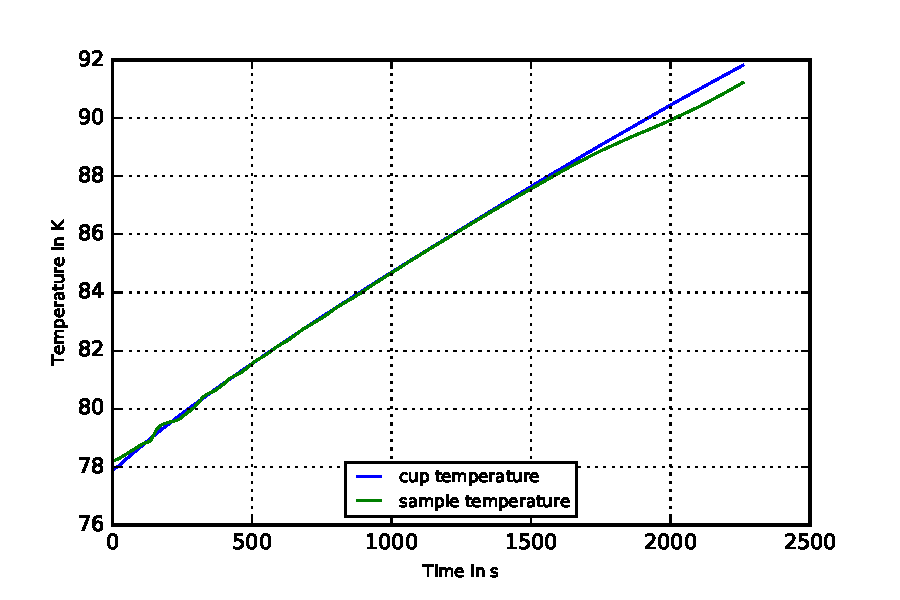
\includegraphics[width = 0.8\textwidth]{fig/latent_raw_j.pdf}
\caption{\label{latent_raw_j}\textbf{Measurement of the temperature around Curie temperature of cup and sample.} A heater was attached to the sample of $0.056\e{mol}$ Dysposioum, which constantly supplied $10.7\e{mW}$ of power.}
\end{figure}
\begin{figure}[h]
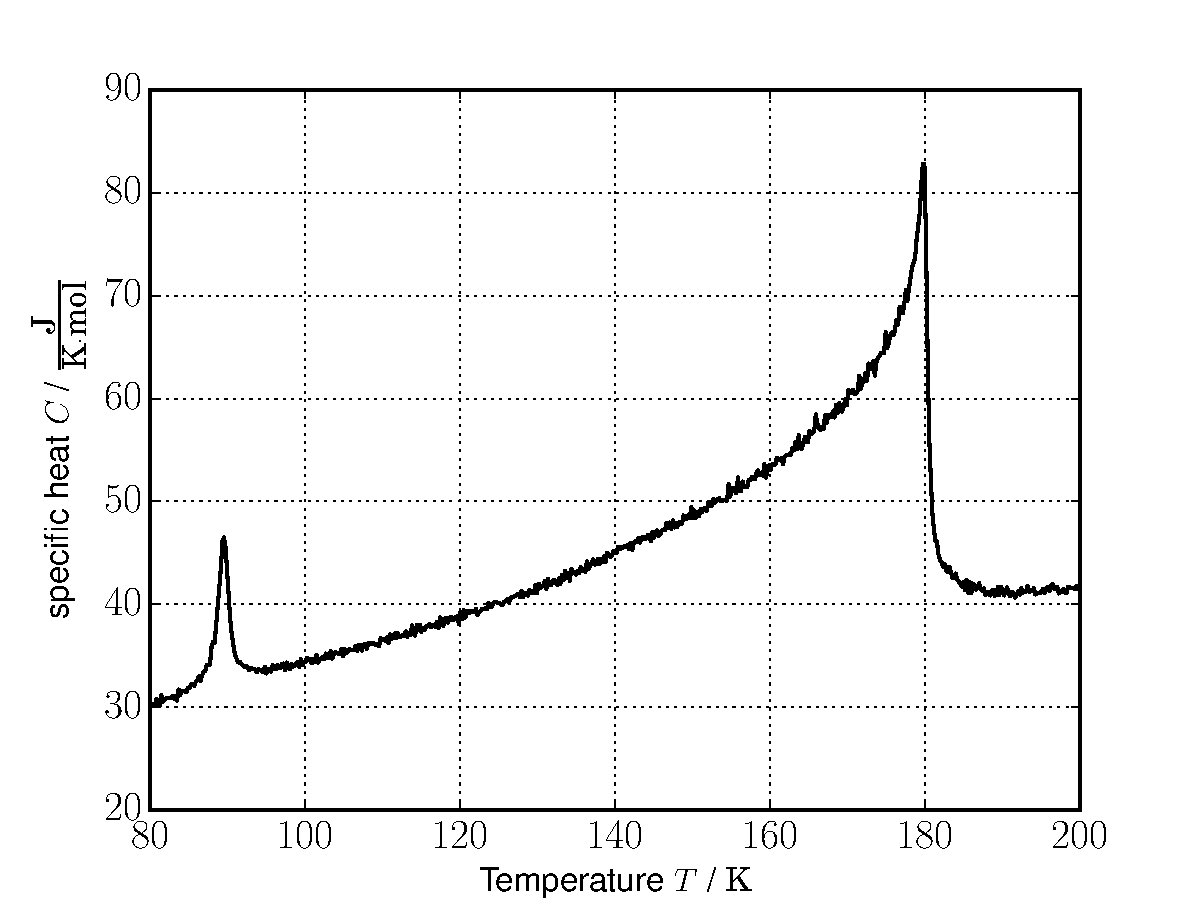
\includegraphics[width = 0.8\textwidth]{fig/data.pdf}
\caption{\label{data}\textbf{Raw set of data for the measurements of the specific heat.} This set of data was recorded while the Dysporium was slowly heated with constant power.}
\end{figure}


\section{Measurements of the latent heat}
The latent heat was measured with two different methods. In the first method the temperature of the sample was measured over time, while heating it with constant power. In the second method the specific heat was measured at different temperatures and the resulting excess heat at the Curie temperature was evaluated.
\subsection{Method one}
\begin{figure}[h]
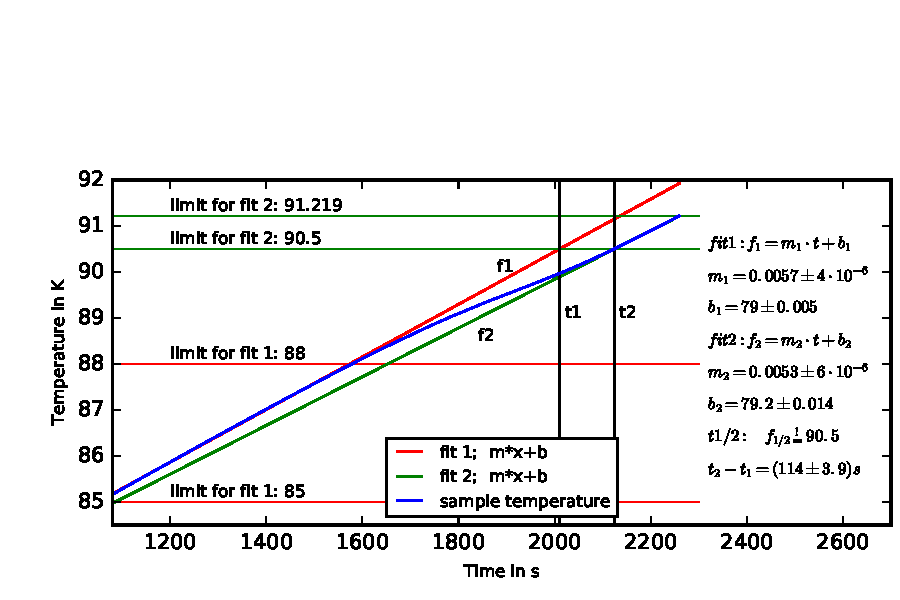
\includegraphics[width = 0.9\textwidth]{fig/latent_j.pdf}
\caption{\label{latent_j}\textbf{Measurement of the latent heat around Curié-Temperature.} Two linear fits (red and green) with its ranges of Rawdata used to fit in matching colors. Latent heat corresponds to the stored energy in the sample while heating between t1 and t2 (black).}
\end{figure}
With the LABView-VI latent.vi the temperature of the cup and the sample was measured while heating up slowly around the Curie temperauture. The raw data is shown in figure \ref{latent_raw_j}. To analyze the latent heat at the phase shift, the drop of the curve was measured. It indicates a lesser rise in temperature over time by the same amount of heat energy. That's why two linear fits where done on the temperature curve of the sample. One before the other after the phase shift, as seen in figure \ref{latent_j} in red and green. The areas of data used to fit these functions are visualized too, as well as the raw data. 

The offset in time of both fits indicates the latent heat, because during this time, the energy of the supplied heat was not used to heat the sample, but rather to enable the phase transformation. The results are the following:
\begin{align}
\Delta t &= t_2-t_1=(114\pm 4)\e{s}\\
\textrm{latent heat} &= P \cdot t / M=10.7\e{mW}\cdot 114\e{s}/0.056\e{mol} \\
\textrm{latent heat} &= (21.8 \pm 0.8)\e{\frac{J}{mol}}
\end{align}
In fact both linear fits should have the same slope which cannot be confirmed by this measurement. This might be caused by the fact, that only a few measurements at temperatures above the phaseshift were recorded. To compensate this, the offset of these slopes where measured at temperatures as high as possible.
\subsection{Method two}
In the second method, the data shown in figure \ref{data} was used. 
At the Curie temperature, the specific heat has a peak which corresponds to the excess heat needed for the phase transition of first order.
The latent heat then corresponds to the integral amount of specific heat, thus a background fit was performed, to determine the excess amount.
The specific heat in the background should show a linear behaviour in temperature, thus a linear fit of the side band regions next to the signal peak at the Curie temperature was performed.
The then resulting excess area in the signal region was calculated.
The results are shown in figure \ref{area}.

The resultung signal area corresponding to the latent heat was calculated to
\[ A = 29.0 \pm 2.9 \e{\frac{J}{mol}}\]
\begin{figure}[h]
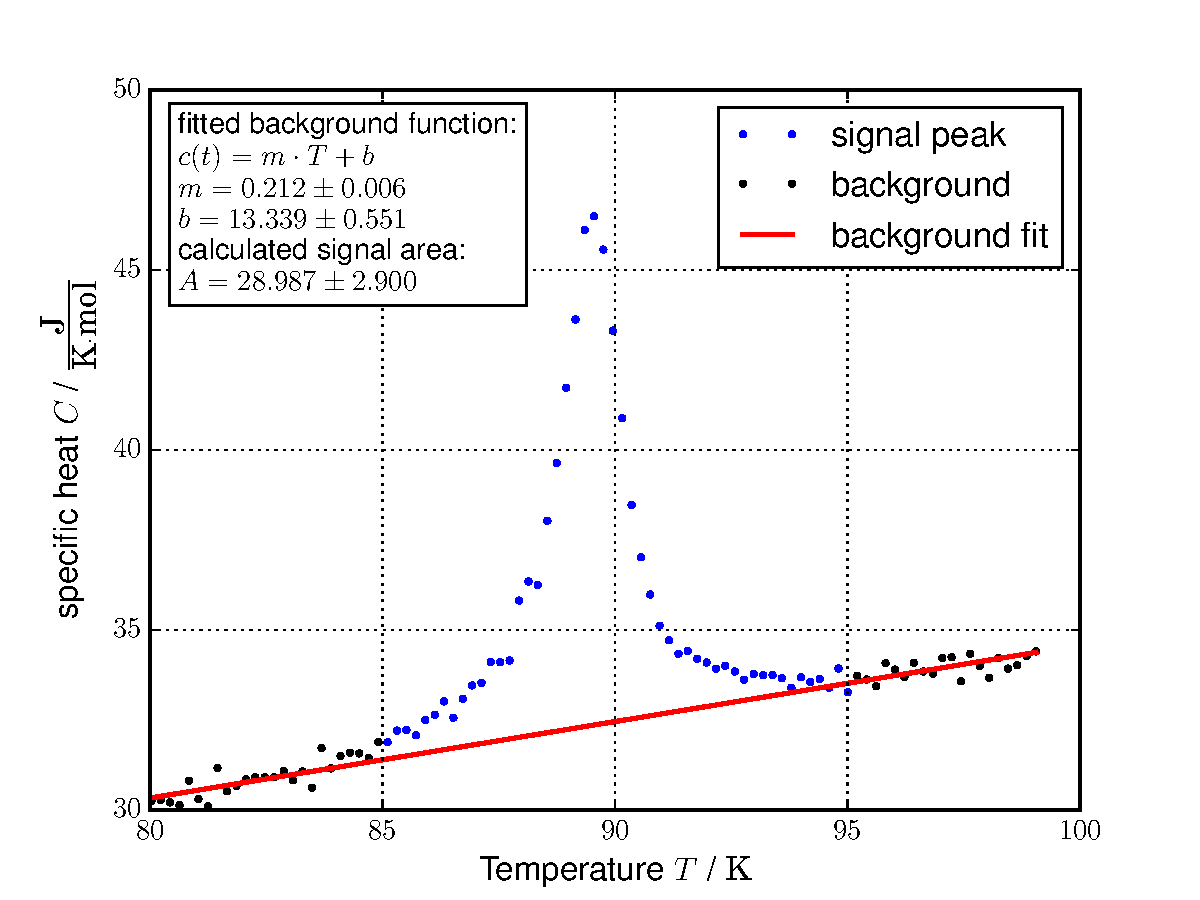
\includegraphics[width = 0.8\textwidth]{fig/latentheat_area.pdf}
\caption{\label{area}\textbf{Specific heat at the Curie temperature.} Shown is the specific heat at temperatures around the Curie temperature. Black corresponds to the background data and blue to the data at the excess peak. The background data was fitted linearly. The calculated area $A$ corresponds to the latent heat needed for the phase shift of first order. The error on the area was propagated from the errors of the background fit.}
\end{figure}
\subsection{Comparison of methods}

\begin{table}[H]
\centering
\caption{\label{latentheattable}\textbf{Summary of the latent heat calculations.}}
\begin{tabular}{r|l|l}
 & latent heat / $\e{\frac{J}{mol}}$ & deviation\\
\midrule
paper & $39.1 \pm 1.5$ & \\
method one & $21,8 \pm 0.8$ & -44 \%\\
method two & $29.0 \pm 2.9$ & -26 \%\\
\midrule
\end{tabular}
\end{table}

Both measured values of the latent heat for the first phase transitions have a deviation of more than $3\sigma$ to the value measured in the paper by Jayasuriya et al.\\
The results of the second method are closer to the measurements of the paper, but also have a higher uncernaity. 

\subsection{Entropy}
The weighted average of the measured values of the latent heat is $Q = 23.4 \pm 3.0 \e{\frac{J}{mol}}$. 
With this value the entropy of the phase transition at the measured Curie temperature $T = 89.55\e{K}$ was calculated
\[S = \frac{Q}{T} = 0.261 \pm 0.03\e{\frac{J}{mol}}\]
Dysporium has an angular momentum of $J = 8$. Therefore its spin entropy is given as
\[S_{spin} = R \ln (2J + 1) = 23.54\e{\frac{J}{mol}}, ~~~~ R = 8.31 \e{\frac{J}{mol}}\]
It becomes apparent, that the entropy gained by the phase transition is very small in comparison with the already present spin entropy. 
\section{Measurements at the Neel temperature}

The phase transition of second order at the Neel temperature was also recorded in the data shown in figure \ref{data}.
From this data, the value of the Neel temperature was calculated to be at
\[T_N = 179,7\e{K}\]
As described in section \ref{neel}, the specific heat at the Neel temperature should follow the following laws
\begin{equation}
\label{fitfunc}
 C_p(T) = \frac{ A^\pm |t|^{-\alpha}}{\alpha} + Et + B, ~~~~ t = \frac{T-T_N}{T_N}
\end{equation}
where $t$ is the reduced temperature, relative to the Neel temperature $T_N$. The coefficient $\alpha$ should be the same for positive and negative $t$, the scaling factors $A^+$ and $A^-$ for the positive and negative $t$ respectively may be different.\\
For further analysis the known background $E t + B$ was substracted. 
The fits of the both ranges for positive and negative $t$ were performed in two ways. In the first method, the functions were fitted directly to the data and in the second method, the data was rescaled logarithmically on both axes and then fitted via the following function:
\[ \ln(C(t)) = \ln \left( \frac{A^\pm}{\alpha}\right) - \alpha \ln (t) \]

\subsection{Direct fit}
\begin{figure}[h]
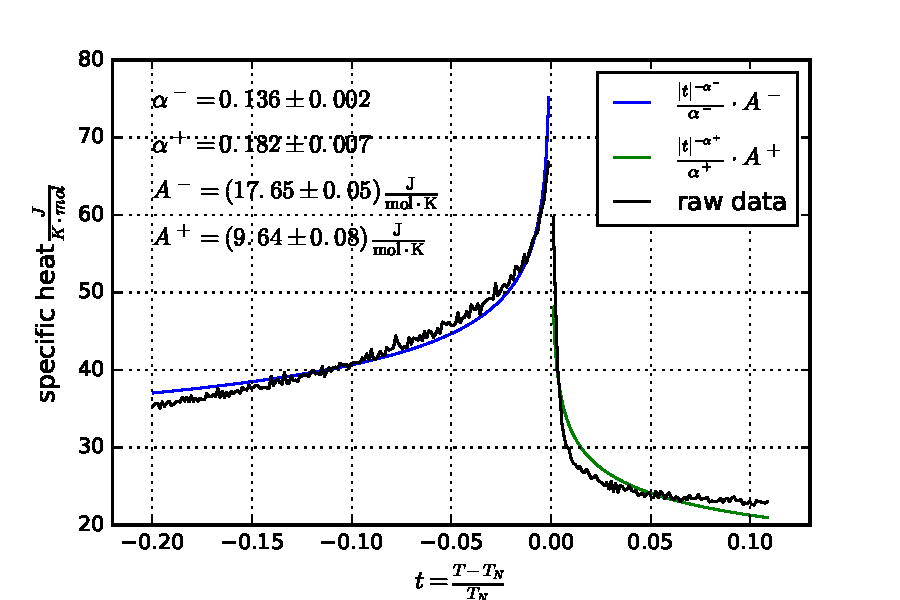
\includegraphics[width = 0.9\textwidth]{fig/specheat_j.pdf}
\caption{\label{specH}\textbf{Reduced temperatures close to the Neel temperature with direct fit.} Both fits were preformed with the function shown in equation \ref{fitfunc}.}  
\end{figure}
Reducing the raw data from figure \ref{data} by the linear background $E + Bt$ and plotting it in respect to the reduced temperature t for $|t|> 0.2$, yields the data shown in figure \ref{specH}. Fitting the mentioned function from equation \ref{fitfunc} leads to the values results shown in the plot.
\begin{align*}
A^- &= 4,04 \pm 0,04 \e{\dfrac{J}{K\cc mol}}\\
A^+ &= 2,54 \pm 0,04 \e{\dfrac{J}{K\cc mol}}\\
\alpha^- &= 0,136 \pm 0,002\\
\alpha^+ &= 0,182 \pm 0,007\\
\end{align*}
In this method a direct fit does not lead to the same value for $\alpha$ on both sides of the phase shift.
\subsection{Double logarithmic fit}
For the second fit method with the double logarithmic fits, the reduced temperatures close the the Neel temperature are shown in figure \ref{neelplot}.



\begin{figure}[h]
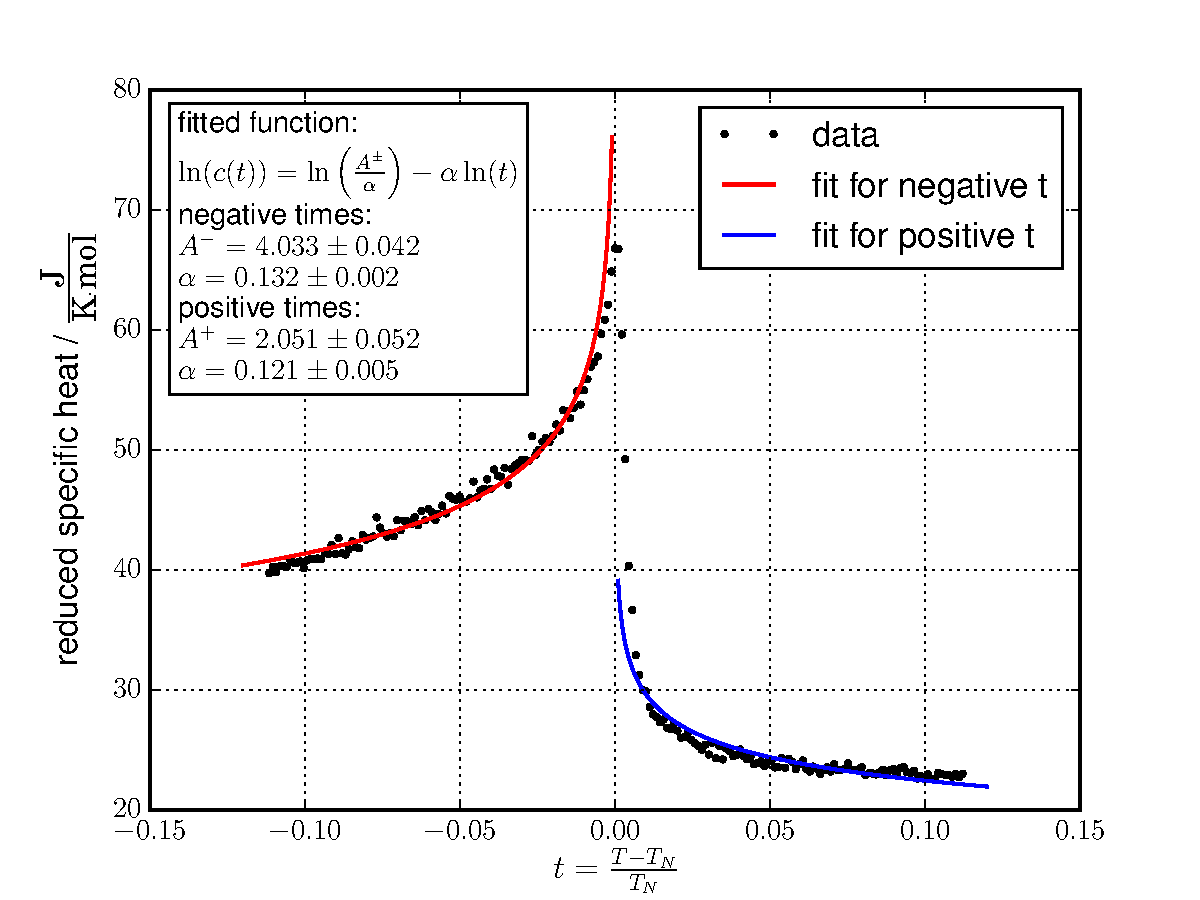
\includegraphics[width = 0.9\textwidth]{fig/loglogfit.pdf}
\caption{\label{neelplot}\textbf{Reduced temperatures close to the Neel temperature with double logarithmic fit.} Additionally to the data the two double logarithmic fits are shown. The red one was performed for $t < 0$ and the blue one for $t > 0$. From the data, the linear background $Et +B$ was substracted before fitting.} 
\end{figure}
The fit values resulting from the double logarithmic fits are the following
\begin{align*}
A^- &= 4,03 \pm 0,04 \e{\dfrac{J}{K\cc mol}}\\
A^+ &= 2,05 \pm 0,05 \e{\dfrac{J}{K\cc mol}}\\
\alpha^- &= 0,132 \pm 0,002\\
\alpha^+ &= 0,121 \pm 0,005\\
\end{align*}
The equality of $\alpha^+$ and $\alpha^-$ can not be confirmed with these fits, as both values have a deviation of at least $2\sigma$.

\subsection{Comparison of fitting methods}
In table \ref{neeltable} the values of $\alpha$ and $A$ for fits at negative and positive $t$ are shown. The results of the both fit methods performed in this experiment were compared with the values shown in TABLE III, Column 3 in the paper. To compare the results with the results of the paper it is to mention, that the the neel temperature determined in this experiment and the paper are not exactly the same. Also  the offset $B$ of the linear background was not constrained in the fits in the paper. Furthermore both fits were performed simultaneously in the paper and thus, only one value for $\alpha$ was calculated, as the fit was constrained to $\alpha^+ = \alpha ^-$.

\begin{table}[H]
\centering
\caption{\label{neeltable}\textbf{Comparison of fit values for both fit methods and the paper.}}
\begin{tabular}{r|lll}

\toprule
Method & direct fit & double log fit & paper \\
\midrule
$\alpha^+$ 						&						&	$0.132 \pm 0.002$&	$0.15\pm 0.04$	\\		
derivation						&						&	$-12.0\e{\%}$		&\\
\midrule
$\alpha^-$ 						&	$0.136 \pm 0.002$	&	$0.121 \pm 0.005$&	$0.15\pm 0.04$	\\
derivation 						&						&	$-19.3\e{\%}$	&\\
\midrule
$A$ / $\e{\frac{J}{K \cc mol}}$ 	&						&	$2.05 \pm 0.05$	&	$1.47\pm 0.16$	\\
derivation 						&						&	$39.5\e{\%}$		&\\
\midrule
$A^+/A^-$ 						&						&	$0.509 \pm 0.013$&	$0.42\pm 0.05$	\\
derivation						&						&	$21.2\e{\%}$		&\\
\midrule
\end{tabular}
\end{table}

\section{Discussion of the specific heat curve}
In the measurements of the specific heat relative to the temperature in figure \ref{rawdata}, both phase transitions could easily be identified. 
Additionally, the specific heat rises with a constant slope at lower temperatures between $80\e{K}$ and about $130\e{K}$. 
At higher temperatures the power law belonging to the phase shift at the Neel temperature interferes with the constant slope.\\
Accodring to the laws of Dulong-Petit, the specific heat should be constant at high temperatures, which could not be confirmed with the measured data, because only data up to temperatures of $200\e{K}$ were recorded.\\
With equation \ref{lowtemp}, the specific heat should follow a distribution proportional to $T^3$ at temperatures below $\Theta_D$, which could not be observed in the measured data, presumably, because the Debye temperature $\Theta_D$ is lower than the lowest recorded temperature of $77\e{K}$.
\end{document}
